\section{2-stage View Matching}\label{section:2stage}

This approach tries to combine both previously presented methods to achieve better results. The first approach works pretty well in many scenes but has one drawback. Since the objects' shapes are mainly ignored, taking into account only the ratio between the volume and the area of the objects, there could be many scenes with similarly placed objects with similar sizes but different shapes. This could lead to many unwanted false positive evaluations. This approach tries to use neural networks presented in section \ref{section:nnMatching} to eliminate these false positives while maintaining most of the advantages of the first approach, described in section \ref{section:hierarchical}.\par

\subsection{Template Building}

The scene representation in this method combines the scene representations from both previously presented techniques. The scene is represented as a set of objects description, as described in section \ref{section:hierarchical}, and simultaneously, the feature extraction described in section \ref{section:nnMatching} is performed. The Final representation is a tuple of the object decomposition and features vector.

\subsection{Template Matching}

As the name of the approach suggests, the matching is performed in two stages. In the first stage, the similarity of the two scenes is calculated the same as in the section \ref{section:hierarchical}. After the similarity is computed, it is compared with a given threshold so that it is predecided, if it is positive or negative. The calculated similarity is returned as a final result if it is negative. If it is positive, the second stage is performed in order to reduce the number of false positives.\par
In the second stage, the feature vectors are compared in the same way as in a section \ref{section:nnMatching}. If the result is higher than another threshold, the result of the first stage is returned. If the result is lower than the threshold, 0 is returned. The whole process is summarized in Figure \ref{fig:twoStageDiagram}.

\begin{figure}[htpb]
    \centering
    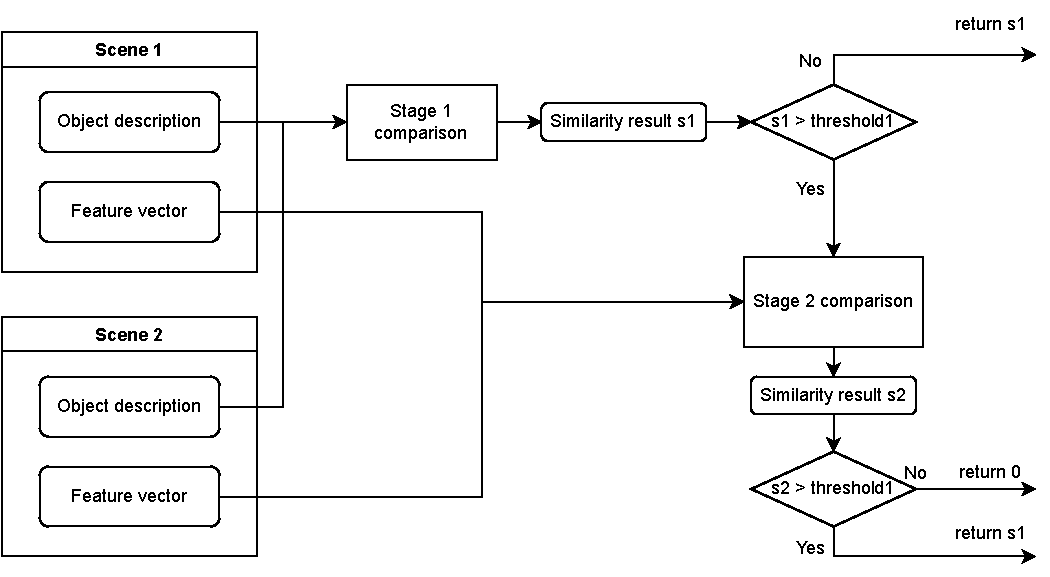
\includegraphics[width=0.8\textwidth]{2stageApproach.pdf}
    \caption{Overview of the two-stage approach} \label{fig:twoStageDiagram}
\end{figure}